\subsection{Definición del problema}

Este trabajo tiene como objetivo el estudio de las redes neuronales recurrentes. No obstante, no solo se centra en el apartado teórico sino que también en el apartado práctico. Por ello, se ha buscado un problema para poder tratar de resolver como ejemplo. El problema que se ha tratado de resolver es la predicción de uso de bicicletas compartidas (\textit{bikesharing}) en la ciudad de Chicago. Como se quiere llevar a cabo una solución usando aprendizaje supervisado, se necesitan previamente una cantidad enorme de datos. Se ha usado Chicago justo por ese motivo, por la facilidad de acceso a los datos públicos necesarios para poder entrenar a la red sin ningún tipo de restricción ni licencia. En concreto se ha descargado el dataset ofrecido por la compañía \textit{Divvy} \cite{divvy}.
\newline
 
Además, el ayuntamiento de Chicago ofrece mapas interactivos \cite{chicagomap} que han sido de gran ayuda para poder estudiar las distintas propiedades de las estaciones al igual que hay multitud de proveedores de datos tanto meteorológicos \cite{chicagoweather} como de otro tipo que también se pueden añadir al \textit{dataset} y así mejorar la precisión del modelo pero que por falta de tiempo y por los resultados obtenidos no se ha podido realizar como se explica en la Sección \ref{future_work}.

\begin{figure}[H]
    \centering
    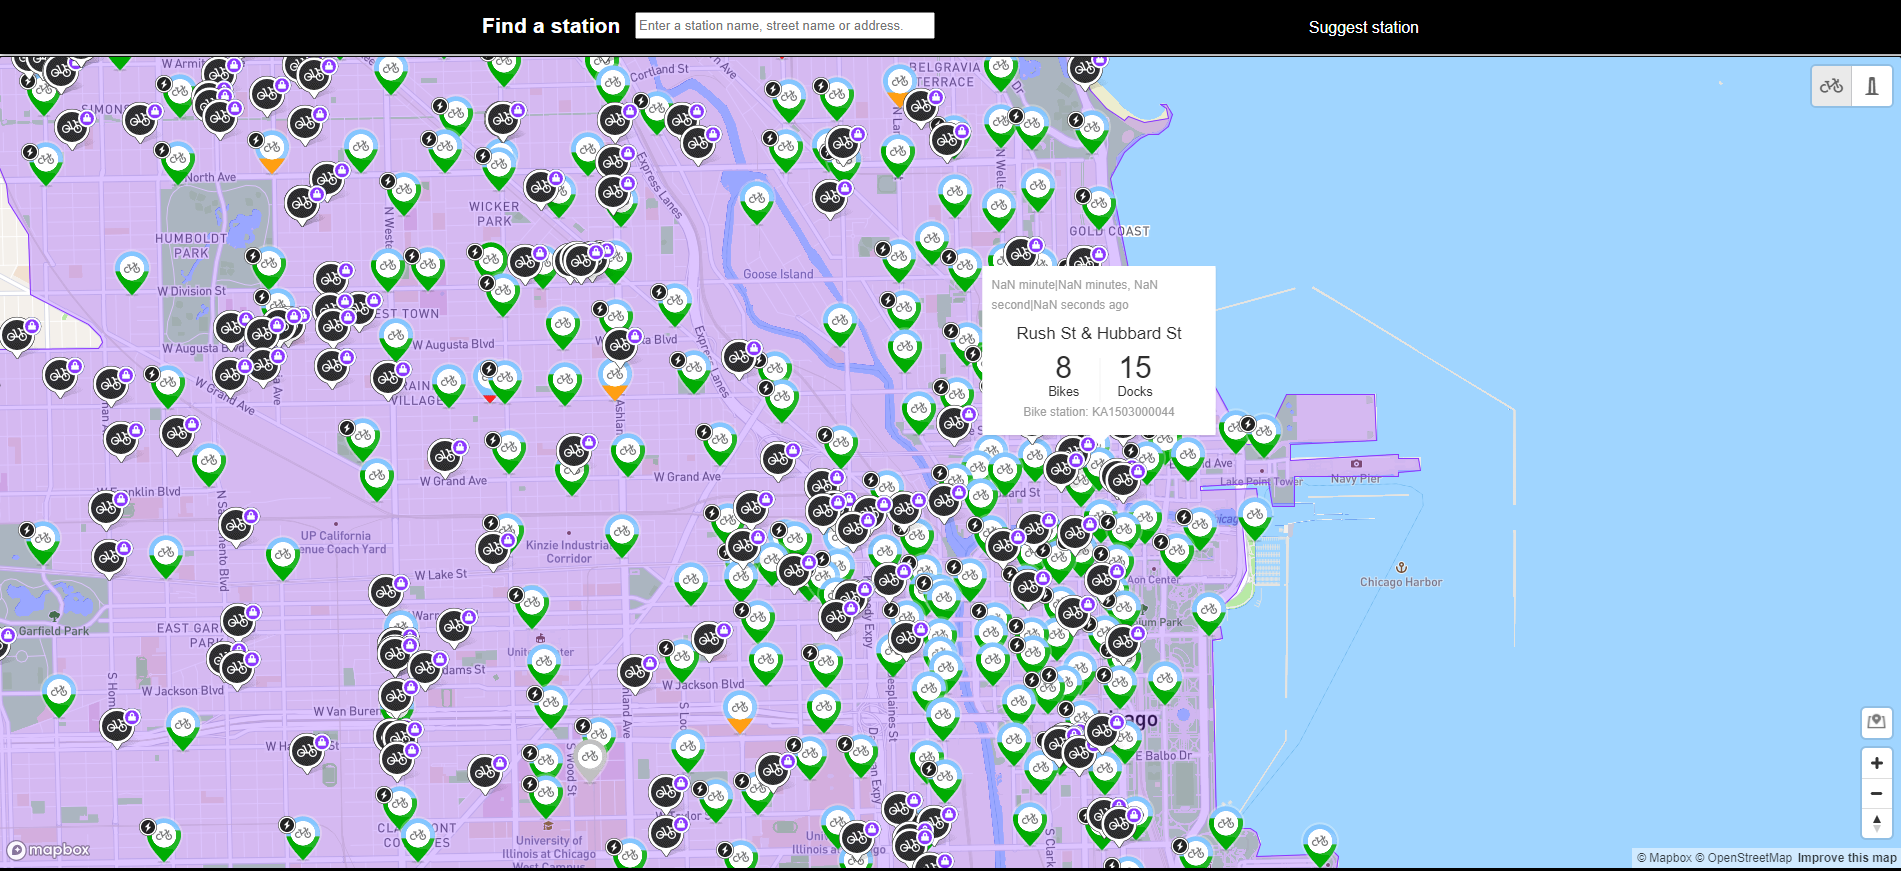
\includegraphics[width=14cm]{images/solution/preprocessing/divvy-map.png}
    \caption{Mapa interactivo de la red de estaciones de alquiler de biciletas en Chicago \cite{chicagomap}}
\end{figure}
